\chapter{Motivácia}

Našim zámerom, bolo vytvorenie funkčnej školskej pomôcky, na štýl experimentu celosvetovo známeho pod názvom Aeropendulum, čo v doslovnom preklade znamená vzdušné kyvadlo. Jedná sa o pomerne jednoduché zariadenie pozostávajúce z niekoľkých častí. Akčným členom tohoto zariadenia je motorček na jednosmerný prúd, ktorý má na rotor pripojené lopatky, ktoré vďaka otáčaniu produkujú ťah. Motorček je zvyčajne upevnený na koniec ľahkej tyčky, ktorá je v mieste otáčania pripevnená k zariadeniu na meranie uhlu pootočenia tyčky. Zariadenie na meranie pootočenia môže byť potenciometer, senzor hallovho javu(efektu), alebo iné \cite{senzor}. V našom prípade budeme používať senzor hall efektu ktorého fungovanie je opísané v časti \ref{Hall}. Zariadenie na meranie uhlu je následne upevnené na podstavec, aby sa motor mohol voľne pohybovať. Podobu modelu Aeropendulum, môžete vidieť na obr. \ref{OBRAZOK 1.1}.

\begin{figure}[!tbh]
	\centering
	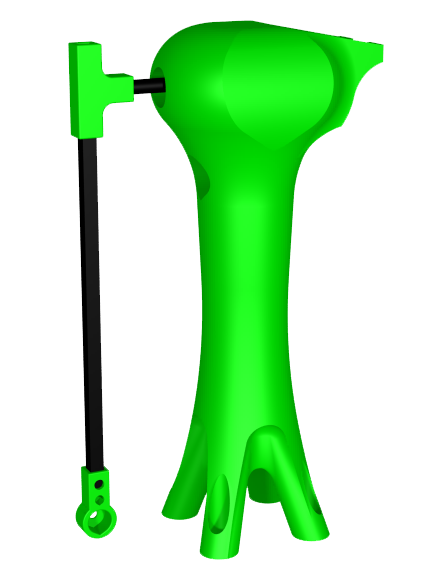
\includegraphics[width=80mm]{obr/AeroCatiaa.png}
	\caption{Model kyvadla, tvorený v programe CATIA.}\label{OBRAZOK 1.1}
\end{figure}

\newpage
Open-source projekt AutomationShield vyvíjaný na ústave Automatizácie, merania a aplikovanej informatiky SJF STU, je zameraný na vývoj hardwarových a softwarových nástrojov určených na vzdelávanie a doplnenie vzdelávacieho procesu. Jadrom celého projektu je tvorba rozširujúcich dosiek (shieldov) vyvíjaných pre populárny typ prototypizačných dosiek s mikrokontrolérmi Arduino, ktoré majú za ciel lepšiu výučbu strojného inžinierstva, mechatroniky a riadenia\cite{Auto}.

Zdrojový kód k AeroShieldu, ako aj ku všetkým modulom AutomationShield, nájdeme na platforme GitHub\cite{Git}, ktorá slúži ako obrovská knižnica kódov, návodov a postupov pre kohokoľvek. Na samostatnej stránke AutomationShield nájdeme zoznam jednotlivých shieldov a to, v akom procese výroby sa nachádzajú. Ku každému shieldu nájdeme jeho podrobnú dokumentáciu, knižnice, zdrojové kódy, ako aj pred programované ukážky fungovania. Tým že GitHub je open-source platforma, dokumenty na stránke môže ktokoľvek upravovať alebo vylepšovať, čo tvorí ideálny priestor pre rozvoj myšlienok a tvorivý proces. Na dokumentoch môže naraz pracovať niekoľko desiatok ľudí, čím sa častokrát mnohonásobne urýchľuje proces tvorby a hľadania chýb.

Ako už bolo spomenuté, hlavnou motiváciou tohoto projektu je nízka dostupnosť a vysoká cena podobných učebných pomôcok. Výučba je preto častokrát až príliš zameraná na memorovanie faktov a teórie, namiesto praktických experimentov a skúseností typu pokus-omyl. Jediný podobný dostupný produkt na kúpu nie ako kit, je Aeropendulum od perzskej značky Real Sim ktoré je na obr.\ref{OBRAZOK 1.2}. Študenti si omnoho rýchlejšie osvoja metódy programovania a automatizácie, pokiaľ majú možnosť experimenty sami tvoriť a skúmať vplyv reálnych výstupov na zvolené vstupy. S úmyslom priniesť širokej verejnosti lacnejšiu a výkonnejšiu alternatívu, vtedajším mnohonásobne drahším a menej výkonným prototypizačným doskám\cite{stamp}, prišla na trh v roku 2005 prototypizačná doska Arduino. Projekt vznikol v Taliansku ako kolaborácia medzi viacerými nadšencami elektrotechniky a programovania, na ktorých čele bol Massimo Banzi.

\begin{figure}[!tbh]
	\centering
	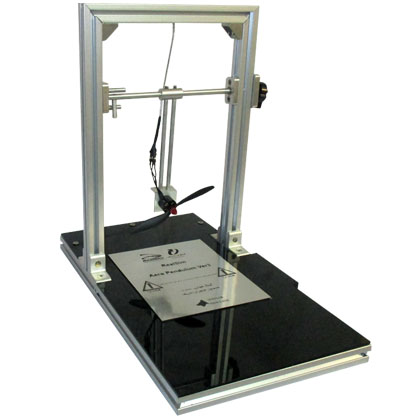
\includegraphics[width=80mm]{obr/pendulum.jpg}
	\caption{{Aeropendulum značky Real Sim\cite{AeroPendulumTeheran}.}}\label{OBRAZOK 1.2}
\end{figure}

\newpage
Veľkou výhodou dosiek Arduino a ich nadstavbových shieldov je fakt, že sú pomerne lacné a majú malé rozmery (Arduino UNO: 68.6*53.4mm\cite{UNO} ). Tieto fakty umožňujú študentom pracovať na experimentoch nielen na pôde školy, ale experimenty si môžu zobrať domov a pracovať na nich aj mimo vyučovacieho procesu. Na správne fungovanie a programovanie dosky nám postačuje len USB kábel a samotná doska. Vzhľadom na nízky počet potrebných súčiastok a fakt, že mikročip arduina je v prípade poruchy jednoducho vymeniteľný \footnote[2]{Tento fakt platí pri mikročipoch typu DIP(Dual in-line package) ktoré stačí jednoducho vytiahnuť z konektora bez použitia spájkovania.}, je ich používanie na školách príjemné a jednoduché. Pre naše účely je vhodná doska Arduino UNO, ktorú môžeme vidieť na obr.\ref{OBRAZOK 1.3}. Na doske sa nachádza 14 digitálnych a 6 analógových pinov. Niektoré piny sú označené špeciálnym symbolom $\sim$. Tieto piny sú schopné produkovať PWM\footnote[3]{Šírková modulácia impulzov alebo PWM je technika na dosiahnutie analógových výsledkov pomocou digitálnych prostriedkov a to, za pomoci striedania dĺžok medzi High a Low stavom resp. zapnutý a vypnutý stav.} signál, ktorý potrebujeme na správne ovládanie motoru kyvadla.

\begin{figure}[!tbh]
	\centering
	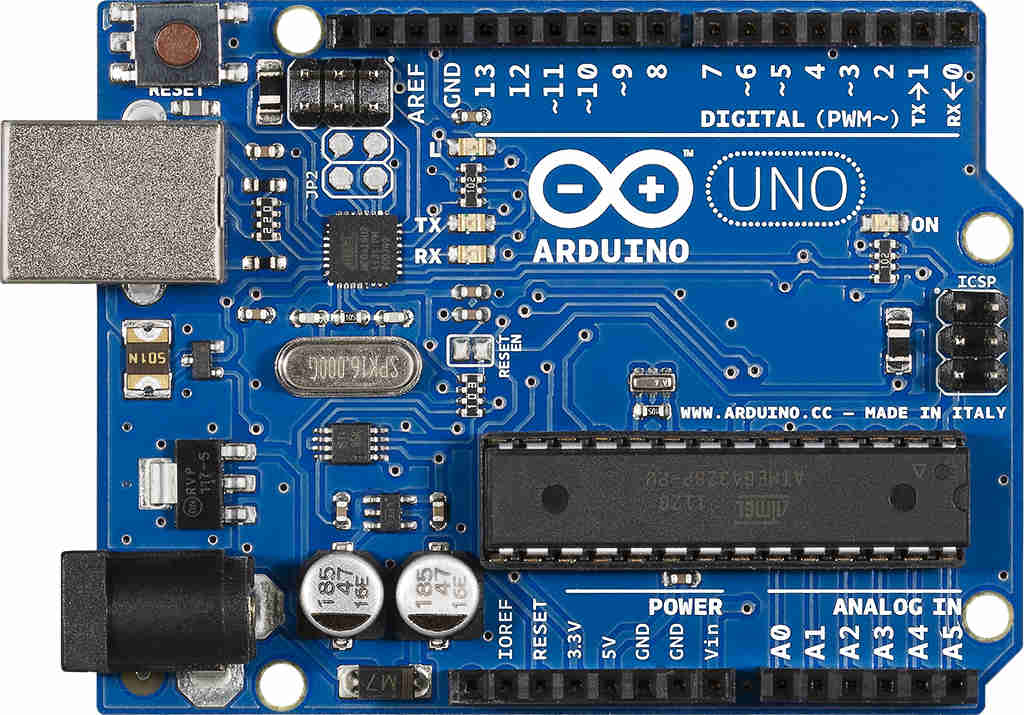
\includegraphics[width=80mm]{obr/arduino.jpg}
	\caption{{Arduino UNO.\cite{UNOFOTO}}}\label{OBRAZOK 1.3}
\end{figure}



